\documentclass[10pt]{beamer}

\usetheme[progressbar=frametitle]{metropolis}
\usepackage{appendixnumberbeamer}

\usepackage{booktabs}
\usepackage[scale=2]{ccicons}

\usepackage{pgfplots}
\usepgfplotslibrary{dateplot}

\usepackage{xspace}
\newcommand{\themename}{\textbf{\textsc{metropolis}}\xspace}

\title{Implementing your  SasModels in Futhark}
\subtitle{It goes much faster}
% \date{\today}
\date{}
\author{Mikkel Storgaard Knudsen}
% \institute{Center for modern beamer themes}
% \titlegraphic{\hfill\includegraphics[height=1.5cm]{logo.pdf}}

\begin{document}

\maketitle

\section{Injecting Futhark into SasModels}

\begin{frame}[fragile]{Basic implementation strategy}
  \begin{itemize}[<+->]
  \item Adding Futhark support to SasModels is very non-invasive.

  \item It is largely a question of adding a third kernel type (FutKernel)
  to exist along the two other available types, PyKernel and GpuKernel.

  SasModels itself behaves the same way no matter the kernel type used;
  as long as the kernel can be initialized and called by SasModels.

  Therefore we can implement FutKernel so it is initialized (and given q-values
  and other details) by SasModels.

  \item When running the computations themselves, the calculations are performed within
  a dynamically loaded, precompiled, highly optimized Futhark kernel, and the
  results are returned to SasModels.
\end{itemize}
  % vis billede af noget diff
\end{frame}
\begin{frame}[fragile]{Basic implementation strategy}

  \begin{figure}
    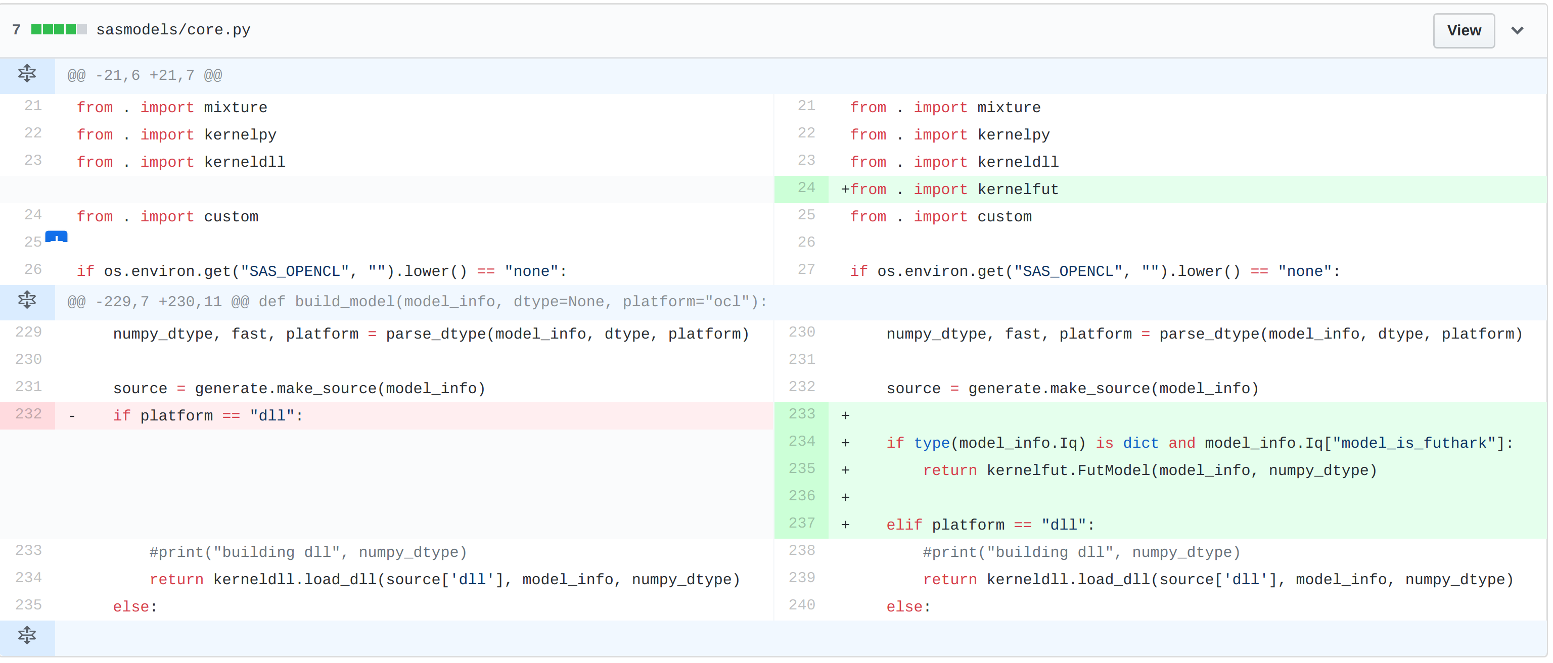
\includegraphics[scale=0.21]{figs/diff.png}
  \caption{The complete contribution to already existing code}
  \end{figure}
\end{frame}
\section{Performance}
\begin{frame}{Average eval time for Line (trivial Python model)}
  \begin{figure}
    \begin{tikzpicture}
      \begin{axis}[
        mbarplot,
        title={1D performance},
        xlabel={nq},
        ylabel={Time in milliseconds},
        width=0.9\textwidth,
        height=3.5cm,
        symbolic x coords={100,500,2500,5000,10000},
        bar width=9pt,
        enlargelimits=0.15,
        ybar=10pt,% configures ‘bar shift’
        bar width=12pt,
        nodes near coords,
        legend style={legend pos=north west}
      ]
      \addplot plot coordinates {(100, 0.24 ) (500, 0.24 ) (2500, 0.26 ) (5000, 0.26 ) (10000, 0.28 )};
      \addplot plot coordinates {(100, 0.93 ) (500, 0.94 ) (2500, 0.97 ) (5000, 0.95 ) (10000, 0.97 )};

      \legend{Current, Futhark}

      \end{axis}
    \end{tikzpicture}
    \begin{tikzpicture}
      \begin{axis}[
        mbarplot,
        title={2D performance},
        xlabel={nq},
        ylabel={Time in milliseconds},
        width=0.9\textwidth,
        height=4cm,
        symbolic x coords={100,500,2500,5000,10000},
        bar width=9pt,
        enlargelimits=0.15,
        ybar=10pt,% configures ‘bar shift’
        bar width=12pt,
        nodes near coords,
        legend style={legend pos=north west}
      ]
      \addplot plot coordinates {(100, 0.31 ) (500, 2.78 ) (2500, 127.01 ) (5000, 501.31 ) (10000, 1970.14 )};
      \addplot plot coordinates {(100, 0.98 ) (500, 1.91 ) (2500, 22.73 ) (5000, 86.03 ) (10000, 338.10 )};

      \legend{Current, Futhark}

      \end{axis}
    \end{tikzpicture}
  \end{figure}
\end{frame}
\begin{frame}{Average eval time for Broad Peak (Python model)}
  \begin{figure}
    \begin{tikzpicture}
      \begin{axis}[
        mbarplot,
        title={1D performance},
        xlabel={nq},
        ylabel={Time in milliseconds},
        width=0.9\textwidth,
        height=3.5cm,
        symbolic x coords={100,500,2500,5000,10000},
        bar width=9pt,
        enlargelimits=0.15,
        ybar=10pt,% configures ‘bar shift’
        bar width=12pt,
        nodes near coords,
        legend style={legend pos=north west}
      ]
      \addplot plot coordinates {(100,0.27) (500,0.30) (2500,0.45) (5000,0.63) (10000,1.22)};
      \addplot plot coordinates {(100,1.22) (500,1.23) (2500,1.23) (5000,1.25) (10000,1.27)};

      \legend{Current, Futhark}

      \end{axis}
    \end{tikzpicture}
    \begin{tikzpicture}
      \begin{axis}[
        mbarplot,
        title={2D performance},
        xlabel={nq},
        ylabel={Time in milliseconds},
        width=0.9\textwidth,
        height=4cm,
        symbolic x coords={100,500,2500,5000,10000},
        bar width=9pt,
        enlargelimits=0.15,
        ybar=10pt,% configures ‘bar shift’
        bar width=12pt,
        nodes near coords,
        legend style={legend pos=north west}
      ]
      \addplot plot coordinates {(100,1.06 ) (500,21.50 ) (2500,675.12) (5000,2686.44 ) (10000,10687)};
      \addplot plot coordinates {(100,1.27 ) (500,2.27 ) (2500,27.48) (5000,103.66 ) (10000,409)};

      \legend{Current, Futhark}

      \end{axis}
    \end{tikzpicture}
  \end{figure}
\end{frame}
\begin{frame}{Average eval time for DAB (trivial OpenCL model)}
  \begin{figure}
    \begin{tikzpicture}
      \begin{axis}[
        mbarplot,
        title={1D performance},
        xlabel={nq},
        ylabel={Time in milliseconds},
        width=0.9\textwidth,
        height=3.5cm,
        symbolic x coords={100,500,2500,5000,10000},
        bar width=9pt,
        enlargelimits=0.15,
        ybar=10pt,% configures ‘bar shift’
        bar width=12pt,
        nodes near coords,
        legend style={legend pos=north west}
      ]
      \addplot plot coordinates {(100, 0.54 ) (500, 0.74 ) (2500, 0.76 ) (5000, 0.74 ) (10000, 0.77 )};
      \addplot plot coordinates {(100, 0.86 ) (500, 0.85 ) (2500, 0.87 ) (5000, 0.87 ) (10000, 0.90 )};

      \legend{Current, Futhark}

      \end{axis}
    \end{tikzpicture}
    \begin{tikzpicture}
      \begin{axis}[
        mbarplot,
        title={2D performance},
        xlabel={nq},
        ylabel={Time in milliseconds},
        width=0.9\textwidth,
        height=4cm,
        symbolic x coords={100,500,2500,5000,10000},
        bar width=9pt,
        enlargelimits=0.15,
        ybar=10pt,% configures ‘bar shift’
        bar width=12pt,
        nodes near coords,
        legend style={legend pos=north west}
      ]
      \addplot plot coordinates {(100, 0.78 ) (500, 1.61 ) (2500, 50.36 ) (5000, 196.19 ) (10000, 771.43 )};
      \addplot plot coordinates {(100, 0.90 ) (500, 1.75 ) (2500, 26.25 ) (5000, 101.59 ) (10000, 402.69 )};

      \legend{Current, Futhark}

      \end{axis}
    \end{tikzpicture}
  \end{figure}
\end{frame}
\begin{frame}{Average eval time for core shell parallelepiped (OpenCL model)}
  \begin{figure}
    \begin{tikzpicture}
      \begin{axis}[
        mbarplot,
        title={1D performance},
        xlabel={nq},
        ylabel={Time in milliseconds},
        width=0.9\textwidth,
        height=3.5cm,
        symbolic x coords={100,500,2500,5000,10000},
        bar width=9pt,
        enlargelimits=0.15,
        ybar=10pt,% configures ‘bar shift’
        bar width=12pt,
        nodes near coords,
        legend style={legend pos=north west}
      ]
      \addplot plot coordinates {(100, 20.88 ) ( 500, 21.19 ) (2500, 21.99) (5000, 22.44 ) (10000, 42.99)};
      \addplot plot coordinates {(100, 2.68 ) (500, 3.67 ) (2500, 8.00 ) (5000, 13.18 ) (10000,23.90 )};

      \legend{Current, Futhark}

      \end{axis}
    \end{tikzpicture}
    \begin{tikzpicture}
      \begin{axis}[
        mbarplot,
        title={2D performance},
        xlabel={nq},
        ylabel={Time in milliseconds},
        width=0.9\textwidth,
        height=4cm,
        symbolic x coords={100,500,2500,5000,10000},
        bar width=9pt,
        enlargelimits=0.15,
        ybar=10pt,% configures ‘bar shift’
        bar width=12pt,
        nodes near coords,
        legend style={legend pos=north west}
      ]
      \addplot plot coordinates {(100, 0.83 ) (500, 2.17 ) (2500, 61.66 ) (5000, 232.32 ) (10000, 986.73 )};
      \addplot plot coordinates {(100, 2.04 ) (500, 2.88 ) (2500, 23.83 ) (5000, 91.87 ) (10000, 357.89 )};

      \legend{Current, Futhark}

      \end{axis}
    \end{tikzpicture}
  \end{figure}
\end{frame}

\section{Future work}
\begin{frame}{Future work}
	SasModels in Futhark is not feature complete yet.
  We still need to implement:
	\begin{itemize}
		\item Polydispersion
		\item Magnetism
		\item Mixture models
		\item Futhark-side refactorings
		\item (various quality-of-life stuff)
	\end{itemize}

  We expect further experiments with more complicated models to show even larger
  performance boosts when using Futhark.
\end{frame}
\end{document}
